\section{Auswertung}
Zunächst soll für die Monozelle der Innenwiderstand und die Leerlaufspannung
bestimmt werden. Dazu werden die Messwerte in Abbildung (\ref{abb:4}) graphisch dargestellt und eine Ausgleichsrechnung,
mithilfe von Python 3.6, durchgeführt. Die Messwerte sind in Tabelle (\ref{tab:1})
gezeigt. Für die Ausgleichsrechnung wird folgende Formel verwendet:

\begin{equation}
  y = -R_i x + U_0
  \label{eq:4}
\end{equation}

Damit ergeben sich die Parameter zu:

\begin{itemize}
  \item $R_i = \SI{16.82(45)}{\ohm}$
  \item $U_0 = \SI{1.63(2)}{\volt}$
\end{itemize}

\begin{table}[H]
  \centering
  \caption{Darstellung der Messwerte der Monozelle.}
  \label{tab:1}
  \begin{tabular}{c c}
    \toprule
    $U_k \, / \, \si{\volt}$ & $ I \, / \, \si{\ampere}$ \\
    \midrule
    0,3  & 0,08  \\
    0,5  & 0,064 \\
    0,75 & 0,054 \\
    0,85 & 0,047 \\
    1    & 0,039 \\
    1,05 & 0,034 \\
    1,1  & 0,03  \\
    1,2  & 0,025 \\
    1,25 & 0,023 \\
    1,3  & 0,02  \\
    \bottomrule
  \end{tabular}
\end{table}

\begin{figure}[H]
  \centering
  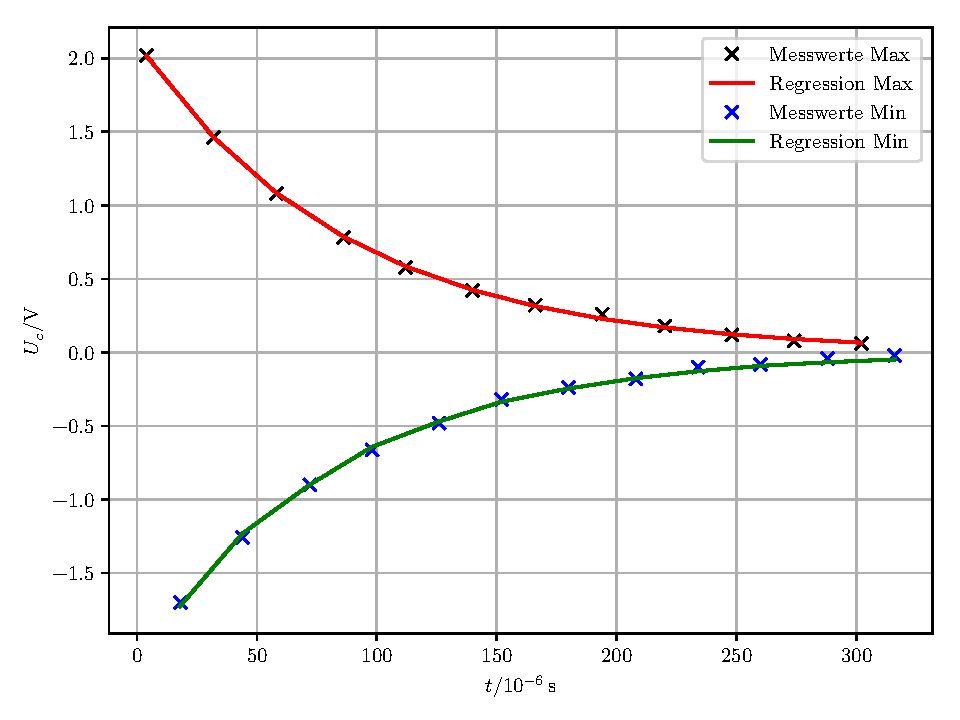
\includegraphics{plot1.py}
  \caption{Graphische Darstellung der Messwerte mit der Ausgleichsgeraden.}
  \label{abb:4}
\end{figure}

Daraufhin wurden die Messungen widerholt, es wurde nur eine Gegenspannung
hinzugeschaltet. Es sollen wieder die Leerlaufspannung und der Innenwiderstand bestimmt
werden. Dazu wird mit der Gleichung (\ref{eq:4}) eine Ausgleichsrechnung durchgeführt.
Eine Graphische Darstellung der Messwerte und der Ausgleichsgeraden sind in Abbildung (\ref{abb:5})
gezeigt. Außerdem sind die Messwerte in Tabelle (\ref{tab:2}) dargestellt.
Durch die Ausgleichsrechnung, die mit Python 3.6 durchgeführt wurde folgt für die Werte:

\begin{itemize}
  \item $-R_i = \SI{18.08(181)}{\ohm}$
  \item $U_0 = \SI{1.53(7)}{\volt}$
\end{itemize}

\begin{table}[H]
  \centering
  \caption{Darstellung der Messwerte der Schaltung mit der Gegenspannung.}
  \label{tab:2}
  \begin{tabular}{c c}
    \toprule
    $U_k \, / \, \si{\volt}$ & $ I \, / \, \si{\ampere}$ \\
    \midrule
    3,1 & 0,091 \\
    2,9 & 0,075 \\
    2,7 & 0,063 \\
    2,6 & 0,055 \\
    2,5 & 0,052 \\
    2,4 & 0,044 \\
    2,3 & 0,040 \\
    2,2 & 0,037 \\
    2,1 & 0,035 \\
    2,0 & 0,032 \\
    \bottomrule
  \end{tabular}
\end{table}

\begin{figure}[H]
  \centering
  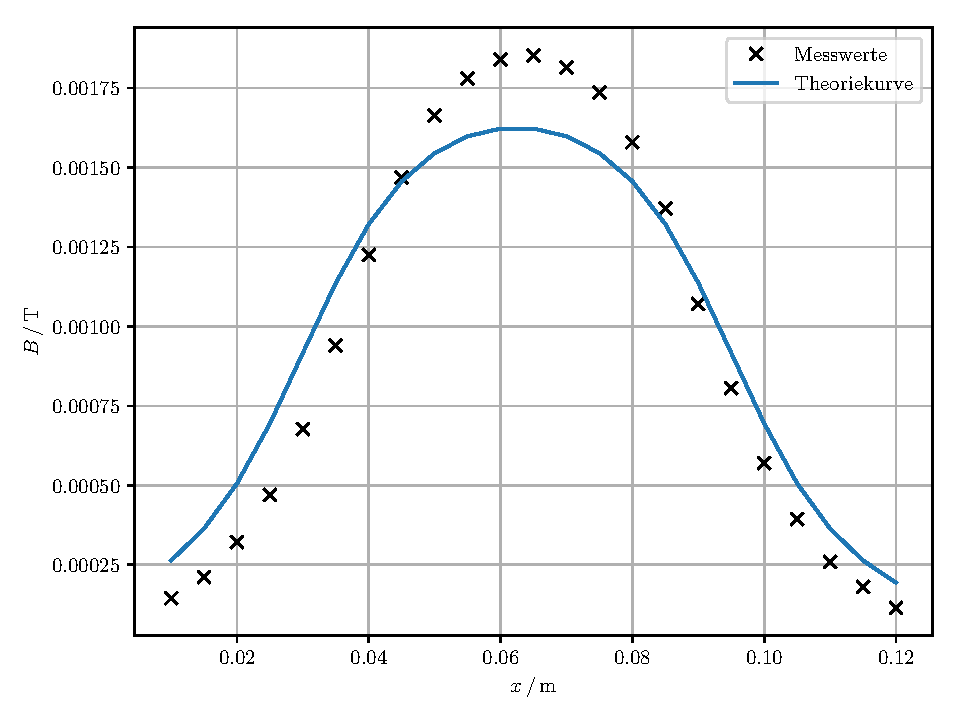
\includegraphics{plot2.py}
  \caption{Graphische Darstellung der Messwerte für die Schaltung mit der Gegenspannung.}
  \label{abb:5}
\end{figure}

Nun wird noch der Innenwiderstand und die Leerlaufspannung von zwei Wechselspannungen bestimmt.
Zunächst für eine Rechteckspannung. Für diesen Fall wird wie zuvor mithilfe der Gleichung
(\ref{eq:4}) eine Lineare Ausgleichsrechnung durchgeführt, welche in der Abbildung
(\ref{abb:6}) graphisch dargestellt ist. Außerdem sind die Messwerte in Tabelle (\ref{tab:3})
auch tabellarisch gezeigt.
Durch die Ausgleichsrechnung ergibt sich für die Werte:

\begin{itemize}
  \item $-R_i = \SI{117.95(188)}{\ohm}$
  \item $U_0 = \SI{3.33(3)}{\volt}$
\end{itemize}

\begin{table}[H]
  \centering
  \caption{Darstellung der Messwerte für eine Rechteckspannung.}
  \label{tab:3}
  \begin{tabular}{c c}
    \toprule
    $U_k \, / \, \si{\volt}$ & $ I \, / \, \si{\ampere}$ \\
    \midrule
    0,5  & 0,024  \\
    0,7  & 0,0225 \\
    1,05 & 0,019  \\
    1,4  & 0,0165 \\
    1,6  & 0,0145 \\
    1,75 & 0,013  \\
    1,95 & 0,012  \\
    2,05 & 0,011  \\
    2,1  & 0,0105 \\
    2,2  & 0,0095 \\
    \bottomrule
  \end{tabular}
\end{table}

\begin{figure}[H]
  \centering
  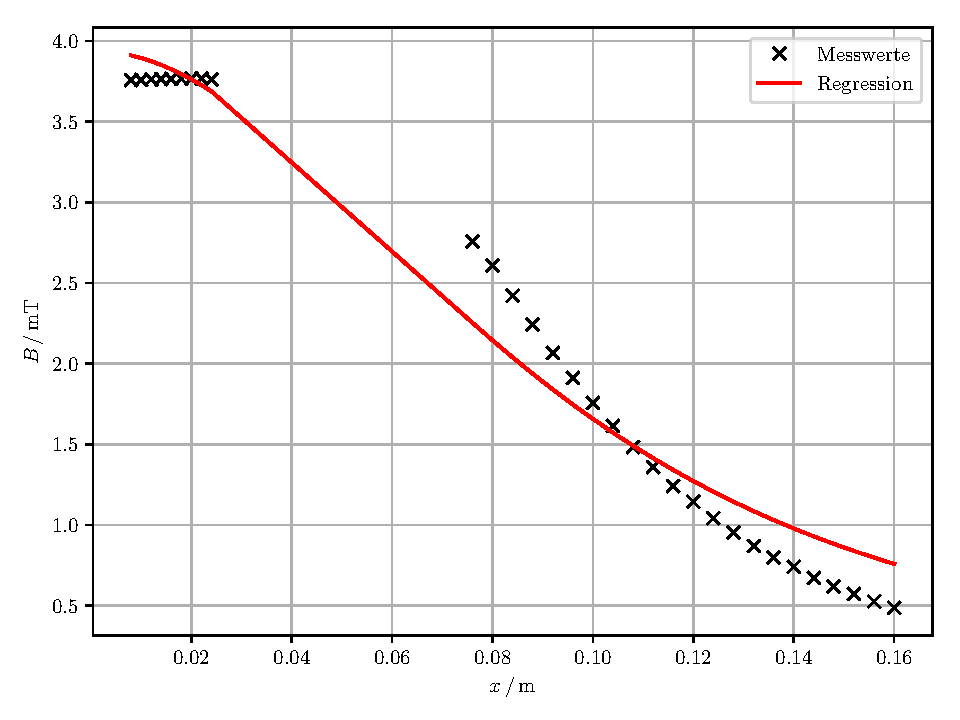
\includegraphics{plot3.py}
  \caption{Graphische Darstellung der Messwerte für eine Rechteckspannung.}
  \label{abb:6}
\end{figure}

Als letztes wird noch der Innenwiderstand und die Leerlaufspannung bei einer Sinusspannung
bestimmt. Das Vorgehen ist analog zu den Messungen zuvor. Die Messergebisse sind
in Abbildung (\ref{abb:7}) graphisch und in Tabelle (\ref{tab:4}) tabellarisch
dargestellt. Die Ergebnisse der Ausgleichsrechnung sind:

\begin{itemize}
  \item $-R_i = \SI{115.21(271)}{\ohm}$
  \item $U_0 = \SI{7.42(6)}{\volt}$
\end{itemize}

\begin{table}[H]
  \centering
  \caption{Darstellung der Messwerte für eine Sinusspannung.}
  \label{tab:4}
  \begin{tabular}{c c}
    \toprule
    $U_k \, / \, \si{\volt}$ & $ I \, / \, \si{\ampere}$ \\
    \midrule
    2,6 & 0,041 \\
    3,6 & 0,033 \\
    4,4 & 0,027 \\
    4,9 & 0,023 \\
    5,1 & 0,02  \\
    5,4 & 0,018 \\
    5,6 & 0,015 \\
    5,8 & 0,014 \\
    6,0 & 0,012 \\
    6,1 & 0,011 \\
    \bottomrule
  \end{tabular}
\end{table}

\begin{figure}[H]
  \centering
  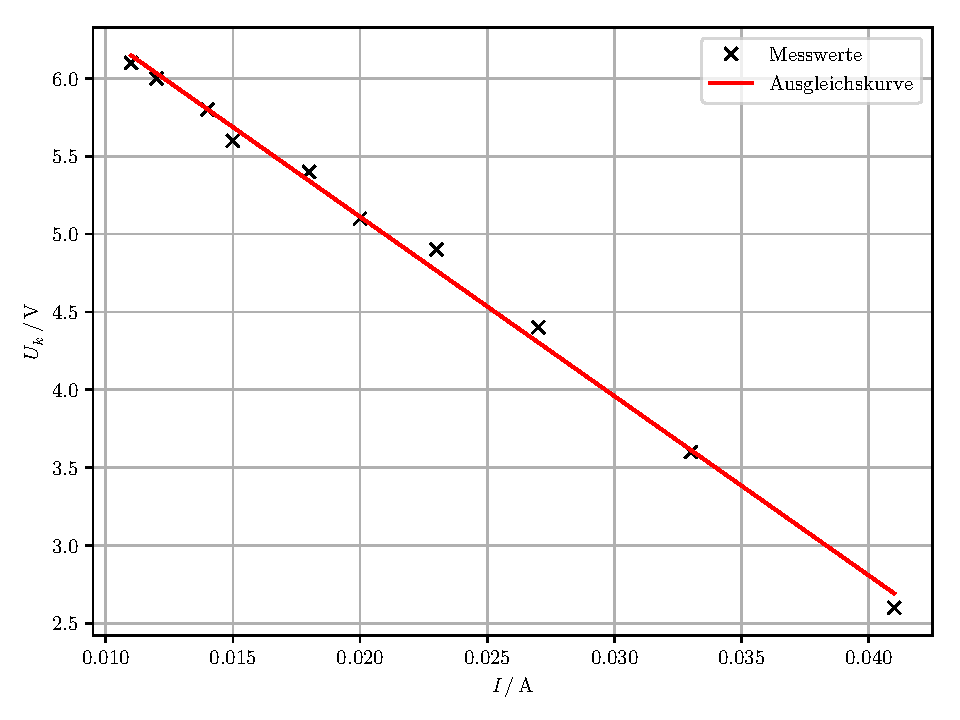
\includegraphics{plot4.py}
  \caption{Graphische Darstellung der Messwerte für eine Sinusspannung.}
  \label{abb:7}
\end{figure}


Zu Begin des Versuchs wurde die Leerlaufspannung der Monozelle gemessen. Diese ergibt sich
zu:

\begin{equation*}
  U_0 = \SI{1.65}{\volt}.
\end{equation*}

Da das reale Voltmeter keinen unendlich großen Widerstand haben kann, er ist in diesem
Fall $R_v = \SI{10^7}{\ohm}$, ergibt sich ein systematischer Fehler bei der Bestimmung
von der Leerlaufspannung. Aus der Gleichung (\ref{eq:2}) und der Gleichung (\ref{eq:1})
folgt die folgende Gleichung für die theoretische Leerlaufspannung.

\begin{equation*}
  U_{0,\text{theo}} = U_0 + \frac{R_i}{R_v} U_0
\end{equation*}

Damit ergibt sich die Formel für den systematischen Fehler:

\begin{equation*}
  \Delta U_0 = \frac{U_{0,\text{theo}} - U_0}{U_0} = \frac{R_i}{R_v}
\end{equation*}

Nun lässt sich der systematische Fehler für die einzelnen Messreihen bestimmen.
Für die Monozelle ergibt sich:

\begin{equation*}
  \Delta U_0 = \SI{1.68(4)e-6}{\percent}.
\end{equation*}

Für die Rechteckspannung:

\begin{equation*}
  \Delta U_0 = \SI{1.179(19)e-5}{\percent}.
\end{equation*}

Für die Sinusspannung:

\begin{equation*}
  \Delta U_0 = \SI{1.152(27)e-5}{\percent}.
\end{equation*}

Die Fehler der systematischen Fehler wurden mit der Gauß´schen Fehlerfortpflanzung
bestimmt:

\begin{equation*}
  \Delta (\Delta U_0) = \sqrt{\left(\frac{1}{R_v} \cdot \Delta R_i\right)}
\end{equation*}

Nun soll die Schaltung in Abbildung (\ref{abb:2}) betrachtet werden, wenn das Voltemeter an
dem Punkt H angeschlossen wird. Dann würde sich ein systematischer Fehler ergeben, der
durch das Amperemeter verursacht wird. Das ideale Amperemeter hat zwar keinen Innenwiderstand,
aber das ist in der realität nicht machbar. Deshalb beeinflusst dieser Innenwiderstand
die Spannungsmessung nach dem Kirchhoffschen Gesetz.\\\\

Als letztes wird die umgesetzte Leistung bei der Monozelle betrachtet. Dazu wird mit der
Gleichung (\ref{eq:1}) aus der gemessenen Spannung und Strom der Belastungswiderstand $R_a$ bestimmt
und damit mithilfe der Gleichung (\ref{eq:3}) die umgesetzte Leistung. Die Ergebnisse sind
in Tabelle (\ref{tab:5}) dargestellt. Außerdem werden diese Werte mit den theoretisch
bestimmten Werten in der Abbildung (\ref{abb:8}) verglichen. Die theoretischen Werte
werden mit der folgenden Gleichung bestimmt:

\begin{equation*}
  N = \frac{U_0^2}{(R_a + R_i)^2} R_a
\end{equation*}

Diese Gleichung lässt sich aus der Gleichung (\ref{eq:3}) herleiten.

\begin{table}[H]
  \centering
  \caption{Errechneten Werte der umgesetzten Leistung.}
  \label{tab:5}
  \begin{tabular}{c c c c}
    \toprule
    $N /\si{\watt}$ & $R_a / \si{\ohm}$ & $N_{\text{theo}} / \si{\watt}$ & Abweichung \, / \, \% \\
    \midrule
    0,0240 & 3,75  & 0,0235 & 2,13 \\
    0,0320 & 7,81  & 0,0342 & 6,43 \\
    0,0405 & 13,89 & 0,0391 & 3,58 \\
    0,0400 & 18,09 & 0,0394 & 1,52 \\
    0,0390 & 25,64 & 0,0377 & 3,45 \\
    0,0357 & 30,88 & 0,0361 & 1,11 \\
    0,0330 & 36,67 & 0,0341 & 3,23 \\
    0,0300 & 48    & 0,0304 & 1,32 \\
    0,0288 & 54,35 & 0,0285 & 1,05 \\
    0,0260 & 65    & 0,0258 & 0,78 \\
    \bottomrule
  \end{tabular}
\end{table}

\begin{figure}[H]
  \centering
  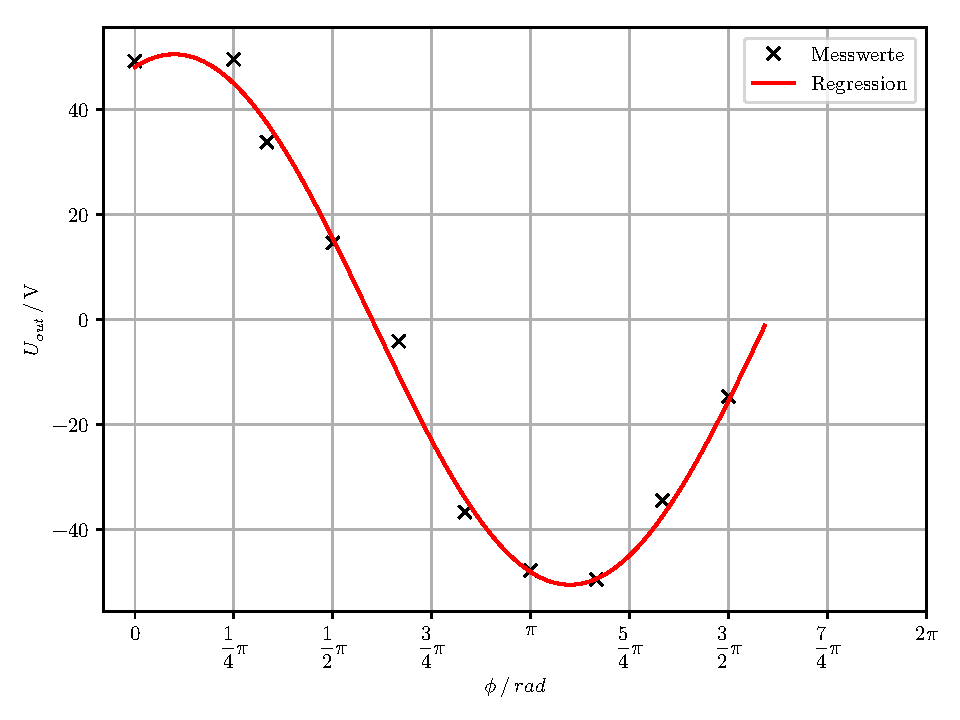
\includegraphics{plot5.py}
  \caption{Graphische Darstellung der umgesetzten Leistung mit den Belastungswiderstand.}
  \label{abb:8}
\end{figure}
